%\documentclass{beamer}
\documentclass[11pt, handout]{beamer}

\usepackage{/home/alex/.latex/stylesheet}
\usepackage{graphicx}
\usepackage{hyperref}
\graphicspath{ {./images/} }

\mode<presentation> {
    \usetheme{default}
    \usecolortheme{seahorse}
    \setbeamertemplate{footline}[page number] % To replace the footer line in all slides with a simple slide count uncomment this line
    \setbeamertemplate{navigation symbols}{} % To remove the navigation symbols from the bottom of all slides uncomment this line
}

\title[Short title]{Investigating Chaos in Schelling's Model} % The short title appears at the bottom of every slide, the full title is only on the title page
\author{Alex Ledger} % Your name
\institute[Reed College] % Your institution as it will appear on the bottom of every slide, may be shorthand to save space
{
Reed College \\ % Your institution for the title page
\medskip
\textit{aledger@reed.edu}% Your email address
}
\date{\today} % Date, can be changed to a custom date

\begin{document}

\begin{frame}
\titlepage 
\end{frame}

\begin{frame}
\frametitle{Overview} 
\end{frame}

\begin{frame}
    \frametitle{Goal}
    \begin{itemize}
        \item Big question: Is society ``chaotic''?
        \item Methodology: Investigate a system that simplifies social relations. 
        \item See if ``chaos'' arises in this simpler model.
    \end{itemize}
\end{frame}

\begin{frame}
    \frametitle{What is chaos?}
    There are three ways that I think about chaos.
    % This is a loaded question with lots of answers.
\end{frame}

\begin{frame}
    \frametitle{1. Sensitivity to Initial Conditions}
    % This is a loaded question with lots of answers.
        \begin{enumerate}
            \item Aka the ``butterfly effect''
            \item If the initial conditions are changed by a marginal amount, how much does that change the output?
            \item e.g. Game of Life: changing one cell in Game of Life can dramatically change the output; hence GoL is chaotic.
            \item e.g. Weather: a slight difference in pressure can lead to dramatically different weather patterns.
        \end{enumerate}

        \begin{figure}
            \center
            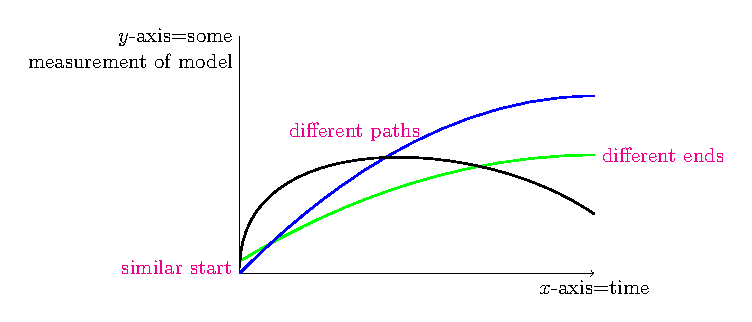
\includegraphics[scale=0.7]{sensitivity_figure/sensitivity_figure.pdf}
        \end{figure}
        \small 
        \href{https://www.youtube.com/watch?v=QXf95_EKS6E}{Double Pendulum Video}
        \normalsize
\end{frame}
\begin{frame}
    \frametitle{2. Unboundedness}
        \begin{enumerate}
            \item A system is unbounded if it grows uncontrollably.
            \item e.g. a cellular automata where it's easy to birth cell and hard to kill cells. Then cells grow indiscrimately into infinitude.
        \end{enumerate}

        \begin{figure}
            \center
            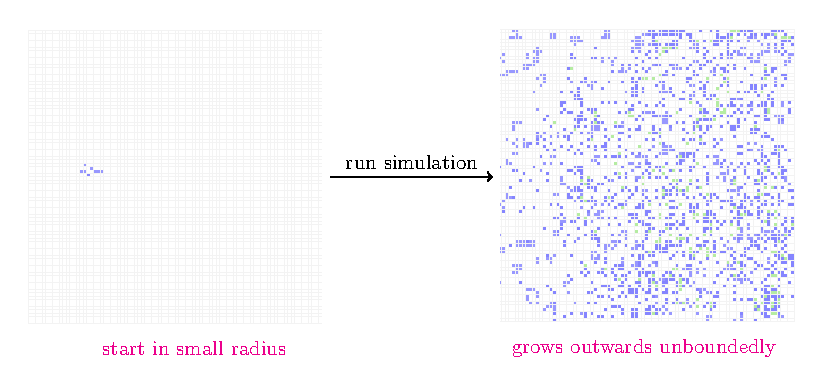
\includegraphics[scale=0.7]{unboundedness_figure/unboundedness_figure.pdf}
        \end{figure}
\end{frame}

\begin{frame}
    \frametitle{3. Unpredictability}
        \begin{enumerate}
            \item More similar to weak emergence than chaos, but still applicable.
            \item Applicable because unpredictability implies that there is no easy way to descrive the behavior of the system (thereby the system is ``chaotic'' in some sense)
                % TODO where should these points go?
            \item Interesting because Economists are so bad at predicting trends. Perhaps we can show that it's because the model is inherently chaotic.
            \item More than showing that the model is chaotic, I want to pinpoint precisely some attributes that make reality chaotic.
        \end{enumerate}
\end{frame}

\begin{frame}
    \frametitle{When, why and how does society exhibit Chaos?}
    When, why and how does society exhibit Chaos?
\end{frame}

\begin{frame}
    \frametitle{Does society exhibit sensitivity to initial conditions?}
    \begin{enumerate}
        \item First you have to define initial conditions: what are society's initial conditions?
        \item Ignore that question: say the initial conditions are the state of society right now.
        \item Then would society, after many years, be significantly different if I had been sitting instead of standing?
        % probably not
        \item It really depends on what condition you change in the initial configuration.
        \item Example 1: 
            \begin{enumerate}
                \item If in one world a baby dies and another the same baby lives, how different are the world?
                \item No idea. Classic argument: what is that baby is Einstein?
                \item However, most likely no major effect.
            \end{enumerate}
    \end{enumerate}
\end{frame}

\begin{frame}
    \frametitle{Does society exhibit unboundedness?}
    \begin{enumerate}
        \item Seems like the answer depends on your scope.
        \item Example 1: A big society - The World.
            \begin{enumerate}
                \item Our population is growing exponentially
                \item We are using more and more resources. Likely to eventually go to Space.
            \end{enumerate}
        \item Example 2: A smaller society - Reed College
            \begin{enumerate}
                \item Reed College is a local ecosystem of social relations.
                \item And it hasn't outgrown its bounds yet. 
                \item I would say the Reed college ecosystem is bounded.
            \end{enumerate}
        \item Worthwhile to ask: what are the key differences between Reed College and all of Mankind that explain the differences in unboundedness?
        \item Perhaps Schelling's Model can elucidate some possible answers.
    \end{enumerate}
\end{frame}

\begin{frame}
    \frametitle{Does society exhibit unpredictability?}
    \begin{enumerate}
        \item Well economics and social trends are notoriously hard to predict. 
        \item So it seems like yeah, to a large extent society is not predictable.
    \end{enumerate}
\end{frame}

\begin{frame}
    \frametitle{Does society exhibit chaos?}
    \begin{enumerate}
        \item {\color{blue} Does society exhibit chaos?}
        \item If it does, why does it exhibit chaos?
        \item If it doesn't, why doesn't it exhibit chaos?
        \item I decided to tackle this question by looking at a ``simpler'' version of society: Schelling's model.
        \item Instead address the question: 
    \item {\color{blue} If, when, and why does Schelling's model exhibit chaos? }
    \end{enumerate}


\end{frame}


\begin{frame}
    \frametitle{Schelling's Model}
    My Implementation of Schelling's model:
    \begin{enumerate}
        \item Two types of people (white and black) located on an $n \times n$ board.
            \begin{itemize}
                \item (picture a chessboard)
            \end{itemize}
        \item Each type of person has a preference for who they like to live near.
        \item If a person's preferences are not met, then they are unhappy.
        \item During each iteration of the model, one unhappy person is randomly selected.
        \item Then that person moves to a random, empty space such that they are happy.
    \end{enumerate}
\end{frame}

\begin{frame}
    \frametitle{Schelling's Model}
    Fixed Parameters to Schelling's Model
    \begin{enumerate}
        \item Two races
        \item Lattice, checkerboard space
        \item Selecting a person to move randomly
    \end{enumerate}
    Variable Parameters to Schelling's Model
    \begin{enumerate}
        \item Vision radius
        \item Moving radius
        \item Selection of who gets to move
        \item Size of board
        \item Edge behavior of board (true edges vs. torus) (TODO add figure)
    \end{enumerate}
        \begin{figure}
            \center
            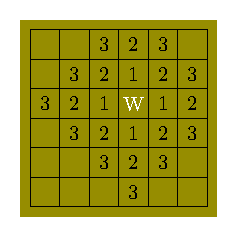
\includegraphics[scale=0.7]{cellular_automata_vision/cellular_automata_vision.pdf}
            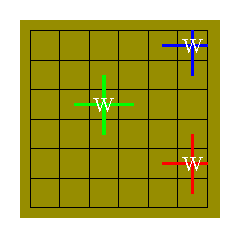
\includegraphics[scale=0.7]{cellular_automata_trueedges/cellular_automata_trueedges.pdf}
            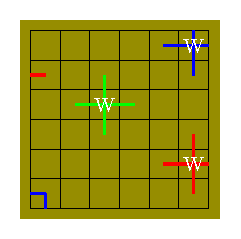
\includegraphics[scale=0.7]{cellular_automata_torus/cellular_automata_torus.pdf}
        \end{figure}
\end{frame}


\begin{frame}
    \frametitle{Justification for Using Schelling's Model}
    % TODO clean up this slide
    % pare it down. I don't think people care too much at this point.
    % probably a more important point to justify in the paper
    \begin{enumerate}
        \item Schelling's model is a simplification of many social relations.
        \item Schelling's model obvious misses a lot of important aspects of social relations, but for the most part those are beside the point.
        \item If Schelling's model under realistic parameters does \emph{not} exhibit chaotic behavior, then
            \begin{enumerate}
                \item Society is not chaotic
                \item Society is chaotic
                    \begin{enumerate}
                        \item Since Schelling's model is a simplification of reality, reality may also be chaotic in the same way.
                    \end{enumerate}
                \item Schelling's Model does not sufficiently model society and we can make no claim about whether society is chaotic.
            \end{enumerate}
        \item Conversely, if Schelling's model under realistic parameters does exhibit chaotic behavior, then there are three possibilities
            % (I like first reason; other two are present for completeness).
            \begin{enumerate}
                \item Society is chaotic, but the chaos stems from phenomena that Schelling's model is not capturing.
                \item Society is not chaotic
                \item Schelling's Model does not sufficiently model society and we can make no claim about whether society is chaotic.
            \end{enumerate}
    \end{enumerate}
\end{frame}

\begin{frame}
    \frametitle{Overview of the Tests}
    \begin{enumerate}
        \item Sensitivity to inital conditions
            \begin{enumerate}
                \item Computed Lyapunov's Exponent
            \end{enumerate}
        \item Unboundedness
            \begin{enumerate}
                \item Idea: initialize to a $20 \times 20$ board but only place people in the middle $8\times 8$ square. Do the people move outwards to the edges of the $20 \times 20$ board?
                    \begin{enumerate}
                        \item Given the model that I decribed, of course they do!
                        \item The people move the random empty spaces.
                    \end{enumerate}
                    \item Change the model such that people only move within their "vision".
                    \item I.e. people have a radius that they use to calculate the composition of their neighbors, and they have a radius that if they are unhappy, they move a random empty square inside of that radius.
                    \item Actually makes the model more realistic, because it's unlikely that people move long, random distances when unhappy; they would be more likely to stay as close as possible while still being happy.
                \item 
            \end{enumerate}
        \item Unpredictability
            \begin{enumerate}
                \item Can a machine learning algorithm predict the behavior of the model.
                \item Inputs: 
                    \begin{enumerate}
                        \item The initial configuration of the board 
                        \item Or the parameters of model
                    \end{enumerate}
                \item Predict:
                    \begin{enumerate}
                        \item The amount of segregation after $n$ trials.
                        \item Whether a given position will be occupied by a black or white person.
                    \end{enumerate}
            \end{enumerate}
    \end{enumerate}
\end{frame}

\begin{frame}
    \frametitle{Lyapunov's Exponents Test and Results}
\end{frame}

\begin{frame}
    \frametitle{Unboundedness Test and Results}
\end{frame}

\begin{frame}
    \frametitle{Unpredictability Test and Results}
\end{frame}

\begin{frame}
    \frametitle{Analysis}
\end{frame}

\begin{frame}
    \frametitle{Conclusions and Further Questions}
\end{frame}


\end{document} 






































